\documentclass[border=10pt,crop=true]{standalone}
\usepackage{tikz}

% $v_i=0$; offset drift $v_o \approx -(V_{\mathrm{of}}/RC)\,t$
% Example: $V_{\mathrm{sat}}=13$ V, $RC=1$ ms, $V_{\mathrm{of}}=5$ mV
% $\Rightarrow t_{\mathrm{sat}}\approx 2.6$ s

\begin{document}
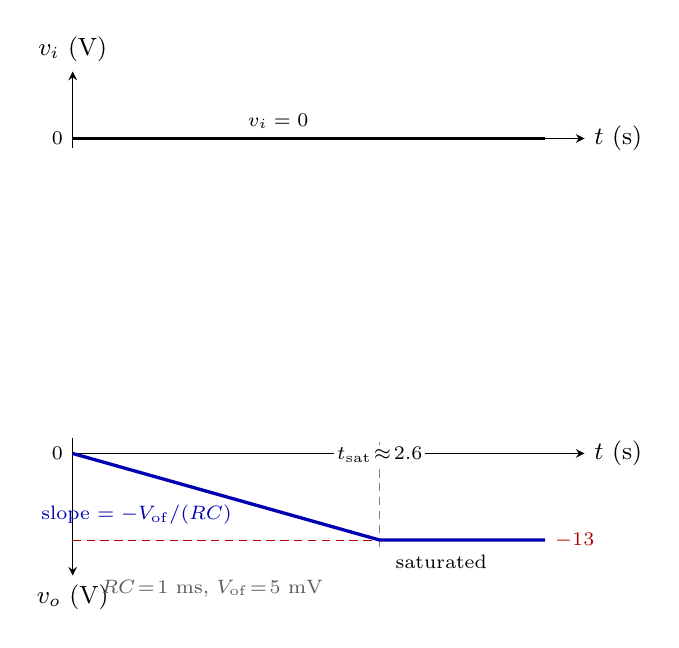
\begin{tikzpicture}[font=\small, >=stealth]
  \def\xs{1.50}       % cm per s
  \def\Tend{4.0}
  \def\Tsat{2.6}
  \def\ViH{0.55}      % top panel height (cm), $v_i=0$
  \def\VoSat{1.10}    % cm for 13 V on bottom panel

  \pgfmathsetmacro{\Xend}{\Tend*\xs}
  \pgfmathsetmacro{\Xsat}{\Tsat*\xs}

  % ----- $v_i$ (zero input) -----
  \begin{scope}[shift={(0,4.0)}]
    \draw[->] (0,0) -- (\Xend+0.5,0) node[right] {$t$ (s)};
    \draw[->] (0,-0.12) -- (0,\ViH+0.30) node[above] {$v_i$ (V)};
    \node[left, font=\scriptsize] at (0,0) {$0$};
    \draw[very thick] (0,0) -- (\Xend,0);
    \node[font=\scriptsize, anchor=west] at (0.35*\Xend,0.22) {$v_i=0$};
  \end{scope}

  % ----- $v_o$ (offset drift to saturation) -----
  \begin{scope}
    \draw[->] (0,0) -- (\Xend+0.5,0) node[right] {$t$ (s)};
    \draw[->] (0,0.2) -- (0,-\VoSat-0.45) node[below] {$v_o$ (V)};
    \node[left, font=\scriptsize] at (0,0) {$0$};
    \draw[densely dashed, red!70!black] (0,-\VoSat) -- (\Xend,-\VoSat);
    \node[right, font=\scriptsize, red!70!black] at (\Xend,-\VoSat) {$-13$};
    \draw[densely dashed, gray] (\Xsat,0.15) -- (\Xsat,-\VoSat-0.15);
    \node[font=\scriptsize, fill=white, inner sep=1pt, anchor=north]
      at (\Xsat,0.12) {$t_{\mathrm{sat}}\!\approx\!2.6$};
    \draw[very thick, blue!70!black] (0,0) -- (\Xsat,-\VoSat) -- (\Xend,-\VoSat);
    \node[font=\scriptsize, blue!70!black, anchor=north east]
      at (0.55*\Xsat,-0.48*\VoSat) {slope $=-V_{\mathrm{of}}/(RC)$};
    \node[font=\scriptsize, anchor=north] at (0.78*\Xend,-\VoSat-0.06)
      {saturated};
    \node[font=\scriptsize, gray!70!black, anchor=north west]
      at (0.04*\Xend,-\VoSat-0.38)
      {$RC\!=\!1$ ms, $V_{\mathrm{of}}\!=\!5$ mV};
  \end{scope}
\end{tikzpicture}
\end{document}
